\begin{problem}[]{Occupy Cal}

You are at Occupy Cal, and the leaders of the protest are deciding whether or not to march on California Hall. The decision is made centrally and communicated to the occupiers via the ``human microphone''; that is, those who hear the information repeat it so that it propagates outward from the center. This scenario is modeled by the following Bayes net:

\vspace{2mm}
\begin{figure}[htp]
\centering
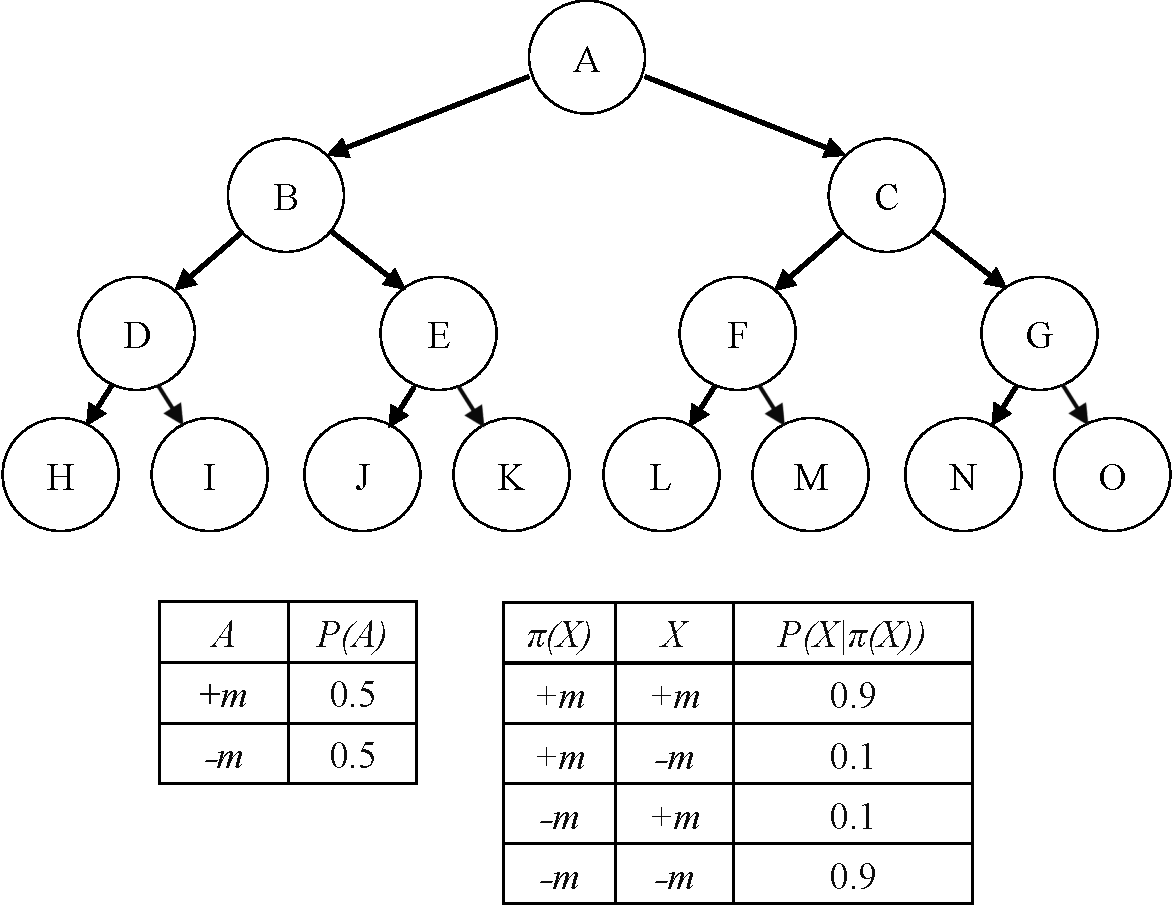
\includegraphics[width=105mm]{figures/tree-labeled-tables-crop.pdf}
\end{figure}
\vspace{2mm}

Each random variable represents whether a given group of protestors hears instructions to march ($+m$) or not ($-m$). The decision is made at $A$, and both outcomes are equally likely. The protestors at each node relay what they hear to their two child nodes, but due to the noise, there is some chance that the information will be misheard. Each node except $A$ takes the same value as its parent with probability 0.9, and the opposite value with probability 0.1, as in the conditional probability tables shown.

\begin{question}[4] Compute the probability that node $A$ sent the order to march ($A = +m$) given that both $B$ and $C$ receive the order to march ($B=+m$, $C=+m$). \\
\fbox{\begin{minipage}[t][4cm][t]{17cm}
\OneA
\end{minipage}}
\end{question}

\begin{question}[4] Compute the probability that $D$ receives the order $+m$ given that $A$ sent the order $+m$. \\
\fbox{\begin{minipage}[t][4cm][t]{17cm}
\OneB
\end{minipage}}
\end{question}

You are at node $D$, and you know what orders have been heard at node $D$. Given your orders, you may either decide to march (\emph{march}) or stay put (\emph{stay}). (Note that these actions are distinct from the orders $+m$ or $-m$ that you hear and pass on. The variables in the Bayes net and their conditional distributions still behave exactly as above.) If you decide to take the action corresponding to the decision that was actually made at $A$ (not necessarily corresponding to your orders!), you receive a reward of $+1$, but if you take the opposite action, you receive a reward of $-1$. \\

\begin{question}[4] Given that you have received the order $+m$, what is the expected utility of your optimal action? (Hint: your answer to part (b) may come in handy.) \\
\fbox{\begin{minipage}[t][5cm][t]{17cm}
\OneC
\end{minipage}}
\end{question}

Now suppose that you can have your friends text you what orders they have received. (Hint: for the following two parts, you should not need to do much computation due to symmetry properties and intuition.)

\begin{question}[4] Compute the VPI of $A$ given that $D = +m$. \\
\fbox{\begin{minipage}[t][5cm][t]{17cm}
\OneD
\end{minipage}}
\end{question}

\begin{question}[4] Compute the VPI of $A$ given that $D = +m$ and $B = -m$. \\
\fbox{\begin{minipage}[t][5cm][t]{17cm}
\OneE
\end{minipage}}
\end{question}

\end{problem}